\thispagestyle{doisongtoanhocnone}
\pagestyle{doisongtoanhoc}
\everymath{\color{doisongtoanhoc}}
\graphicspath{{../doisongtoanhoc/pic/}}
\blfootnote{$^1$\color{doisongtoanhoc}Viện Toán học.}
\begingroup
\AddToShipoutPicture*{\put(0,616){\includegraphics[width=19.3cm]{../bannerdoisong}}}
\AddToShipoutPicture*{\put(64,500){\includegraphics[scale=0.95]{../tieude.pdf}}}\centering
\endgroup

\vspace*{210pt}


\begin{multicols}{2}	
	Từ ngày $08/08/2023$ đến ngày $12/08/2023$, tại Trường Đại học Sư phạm -- Đại học Đà Nẵng, Hội Toán học Việt Nam đã chủ trì và phối hợp với Viện nghiên cứu cao cấp về Toán, Trường Đại học Sư phạm -- Đại học Đà Nẵng, Trường Đại học Khoa học Tự nhiên -- Đại học Quốc gia Hà Nội, Viện Toán học -- Viện Hàn lâm Khoa học và Công nghệ Việt Nam tổ chức Hội nghị Toán học toàn quốc lần thứ X.
	\vskip 0.1cm
	Hội nghị Toán học toàn quốc là hoạt động khoa học lớn nhất của cộng đồng Toán học Việt Nam, được tổ chức $5$ năm một lần. Hội nghị là diễn đàn để các nhà nghiên cứu, ứng dụng và giáo dục toán học trên cả nước trình bày những thành tựu nghiên cứu của mình trong vòng $5$ năm gần đây. Đây cũng là dịp để cộng đồng Toán học Việt Nam, cả trong và ngoài nước, tham gia trao đổi và đóng góp ý kiến về những vấn đề thời sự, cấp thiết đối với sự phát triển Toán học của nước nhà. Tham dự Hội nghị năm nay có hơn $900$ đại biểu đến từ các viện nghiên cứu, học viện, trường đại học và trường trung học phổ thông trên mọi miền đất nước, trong đó có $3$ đại biểu nước ngoài và $90$ nhà toán học Việt Nam đang làm việc ở nước ngoài. Hai nội dung chính của Hội nghị Toán học toàn quốc năm nay là Hội nghị khoa học và Đại hội Đại biểu Hội Toán học Việt Nam lần thứ IX.
	\begin{figure}[H]
		\vspace*{-5pt}
		\centering
		\captionsetup{labelformat= empty, justification=centering}
		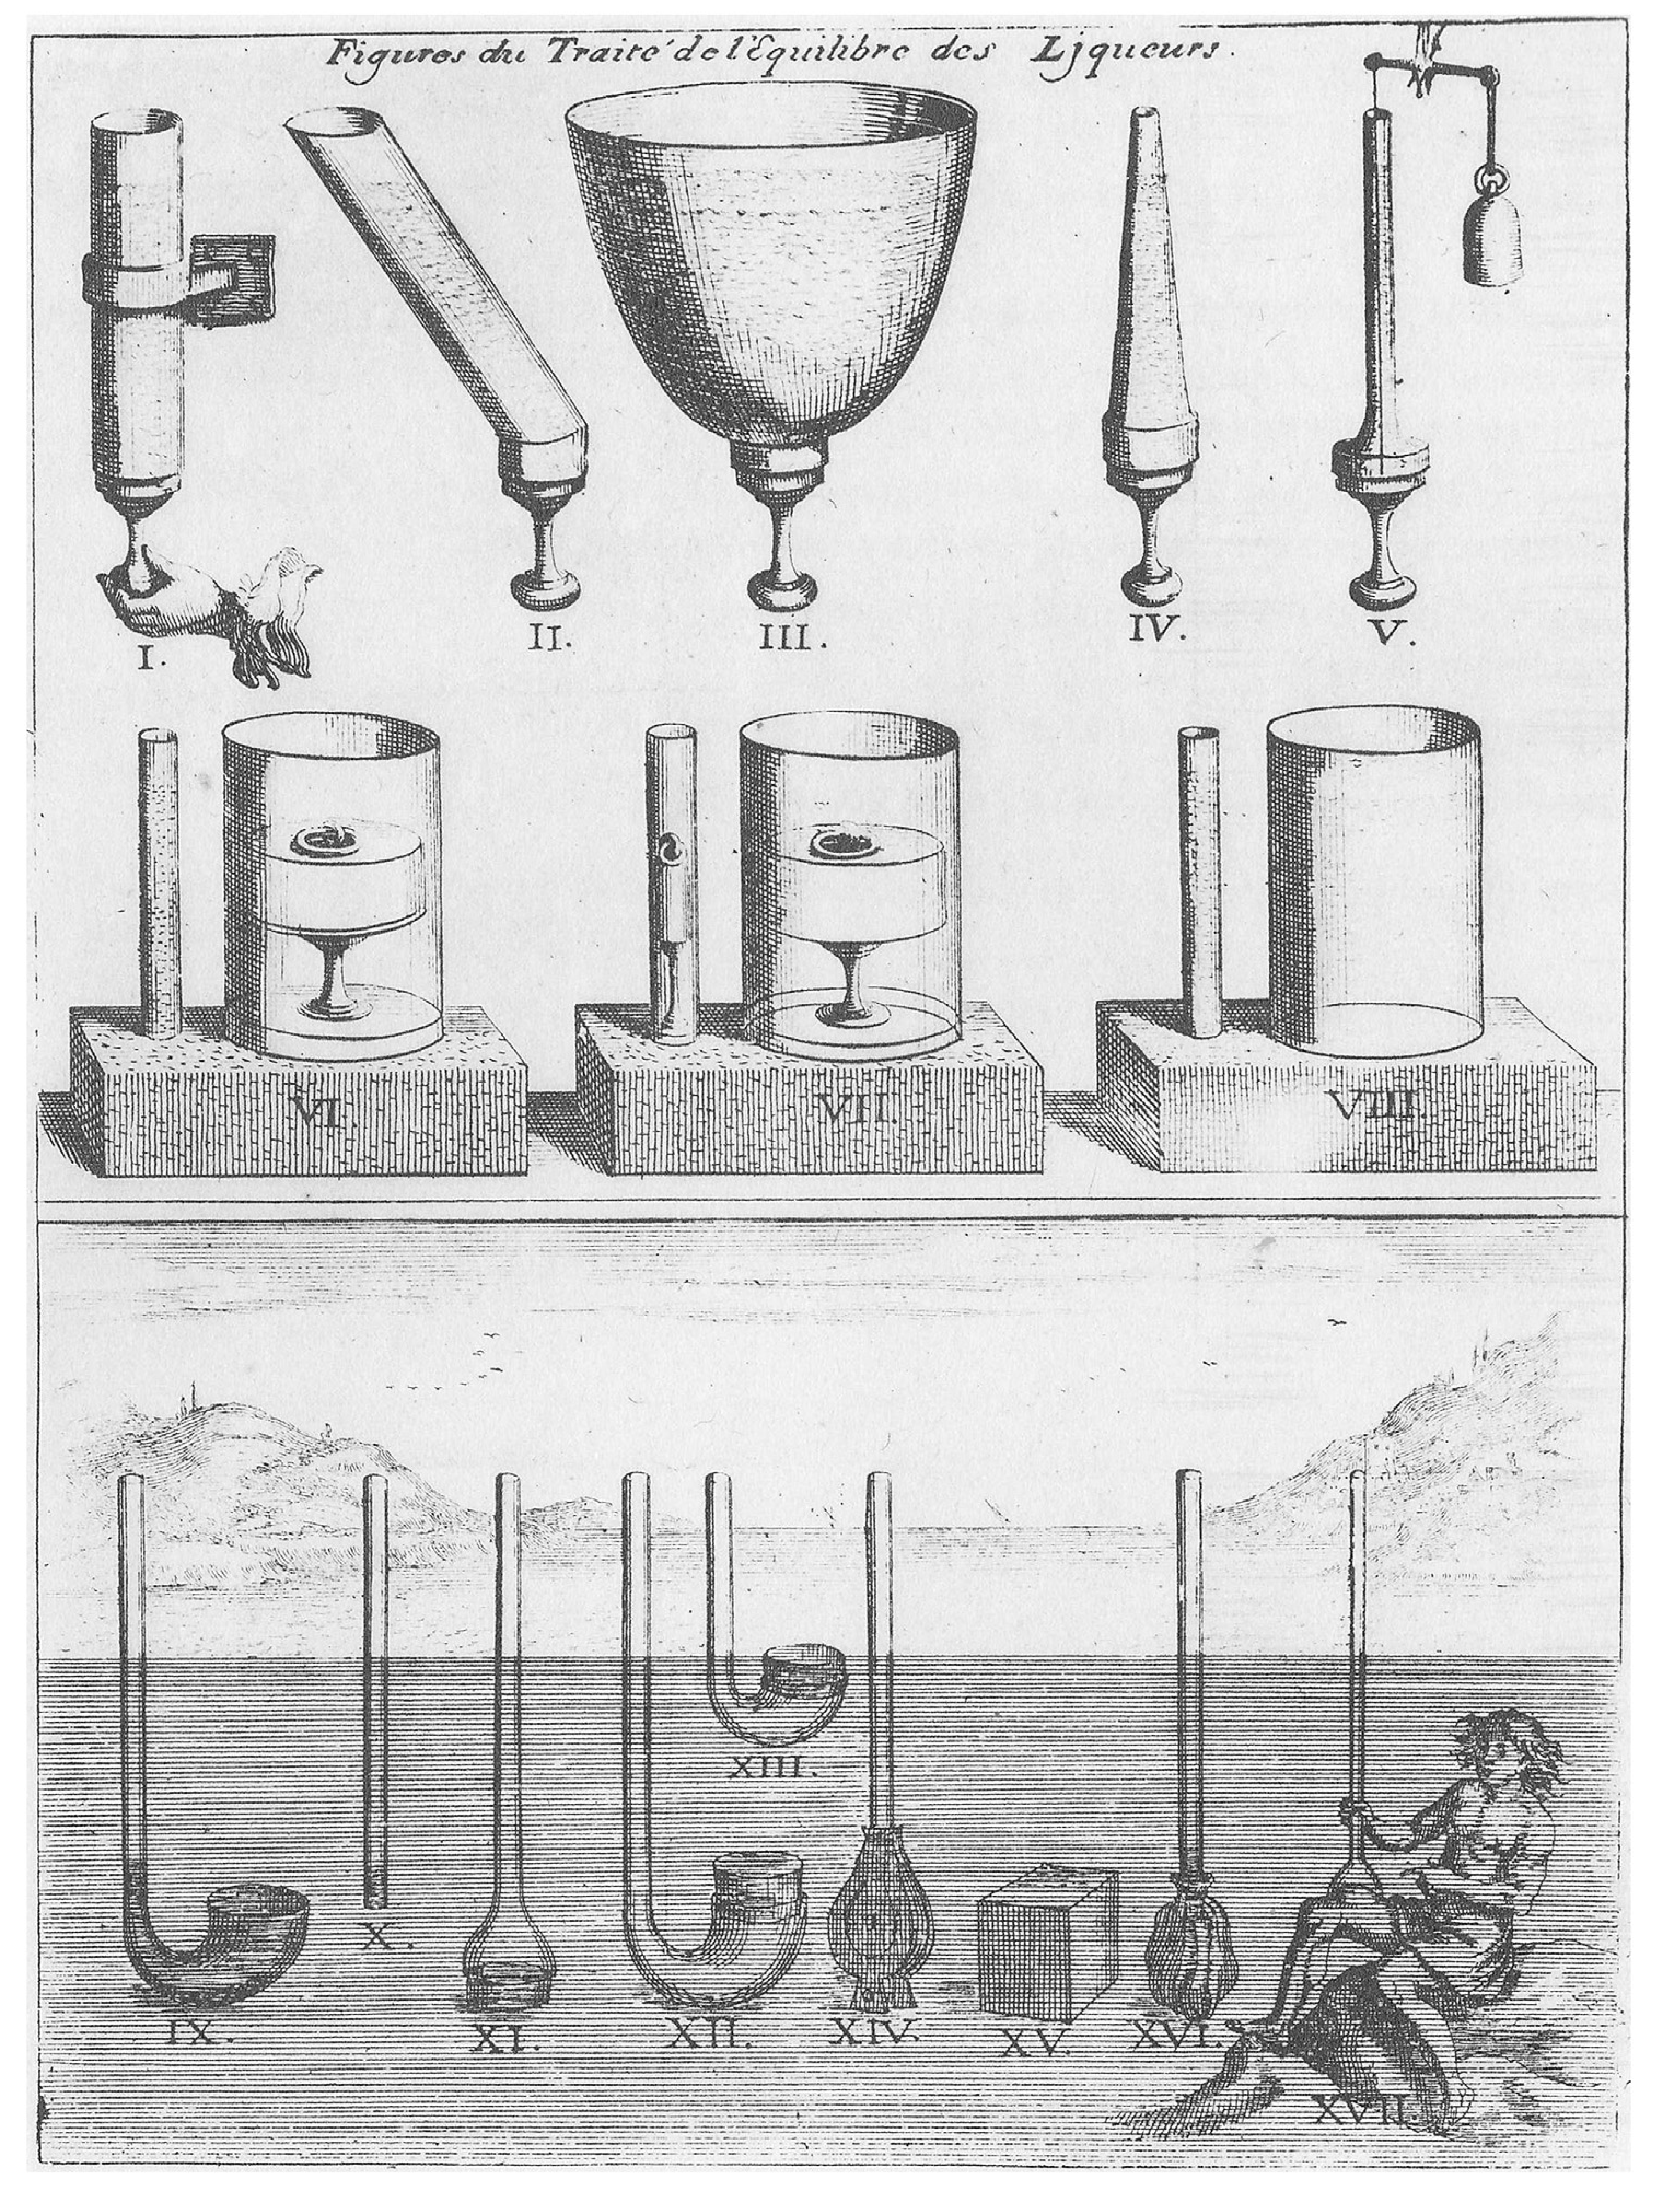
\includegraphics[width= 1\linewidth]{2}
		\caption{\small\textit{\color{doisongtoanhoc}GS. TSKH. Vũ Hoàng Linh Chủ tịch Hội Toán học Việt Nam nhiệm kỳ $2023-2028$.}}
		\vspace*{-10pt}
	\end{figure}
	Phần Hội nghị khoa học đã diễn ra với $7$ phiên toàn thể và $224$ phiên báo cáo thuộc $10$ tiểu ban: Đại số -- Lý thuyết số, Hình học -- Tôpô, Giải tích, Phương trình vi phân và Hệ động lực, Toán rời rạc và Cơ sở Toán học của Tin học, Tối ưu và Lý thuyết Điều khiển, Xác suất -- Thống kê -- Khoa học dữ liệu, Giải tích số và Ứng dụng Toán học, Giảng dạy và Lịch sử Toán học, Phương trình Đạo hàm riêng. Ban tổ chức đã mời $7$ nhà toán học đọc báo cáo mời tại các phiên toàn thể:
	\vskip 0.1cm
	$1.$ Đinh Tiến Cường (National University of Singapore): \textit{Dynamics of complex Hénon maps};
	\vskip 0.1cm
	$2.$ Đinh Dũng (Đại học Quốc gia Hà Nội): \textit{Sparsity in uncertainty qualification for PDEs with Gaussian random field inputs};
	\vskip 0.1cm
	$3.$ Nguyễn Văn Hoàng (Trường Đại học FPT): \textit{Stability estimates for the sharp Sobolev type inequalities};
	\vskip 0.1cm
	$4.$ Đoàn Thái Sơn (Viện Toán học -- Viện Hàn lâm Khoa học và Công nghệ Việt Nam): \textit{Random dynamical systems};
	\vskip 0.1cm
	$5.$ Phạm Tiến Sơn (Trường Đại học Đà Lạt): \textit{Polynomial optimization from the viewpoint of singularity theory};
	\vskip 0.1cm
	$6.$ Nguyễn Duy Tân (Đại học Bách khoa Hà Nội): \textit{On the Massey vanishing conjecture in Galois cohomology of fields};
	\vskip 0.1cm
	$7.$ Vũ Hà Văn (Yale University, Mỹ): \textit{Random matrices and data recovery}.
	\begin{figure}[H]
		\vspace*{-5pt}
		\centering
		\captionsetup{labelformat= empty, justification=centering}
		\includegraphics[width= 1\linewidth]{3}
		\caption{\small\textit{\color{doisongtoanhoc}PGS. TS. Đoàn Trung Cường Phó Chủ tịch kiêm Tổng Thư ký Hội Toán học Việt Nam nhiệm kỳ $2023-2028$.}}
		\vspace*{-10pt}
	\end{figure}
	Đã có $70$ báo cáo mời tiểu ban và $413$ báo cáo ngắn được trình bày tại các phiên báo cáo tiểu ban. Các báo cáo khoa học được trình bày có chủ đề đa dạng, giới thiệu những hướng nghiên cứu thời sự và các thành tựu nghiên cứu gần đây của các nhà toán học Việt Nam. Có nhiều báo cáo trong số đó là của các nhà toán học trẻ có thành tích nghiên cứu xuất sắc. Đặc biệt, với $110$ báo cáo được trình bày bởi các nhà toán học nữ, đây là kỳ hội nghị có số lượng đại biểu nữ trình bày báo cáo cao nhất từ trước tới nay.
	\vskip 0.1cm
	Trong chương trình Hội nghị, Đại hội Đại biểu Hội Toán học Việt Nam lần thứ IX đã được tổ chức vào ngày $10/08/2023$. Các đại biểu đã bầu ra Ban chấp hành Hội Toán học Việt Nam khóa IX (nhiệm kỳ $2023-2028$), bầu trực tiếp Chủ tịch và Tổng thư ký của Hội. Ban Chấp hành mới đã họp ngay trong chiều ngày $10/08/2023$ và quyết định phân công như sau.
	\vskip 0.1cm
	$1.$ GS. TSKH. Vũ Hoàng Linh (Trường Đại học Khoa học Tự nhiên -- Đại học Quốc gia Hà Nội): \textit{Chủ tịch}.
	\vskip 0.1cm
	$2.$ PGS. TS. Đoàn Trung Cường (Viện Toán học – Viện Hàn lâm Khoa học và Công nghệ Việt Nam): \textit{Phó Chủ tịch kiêm Tổng thư ký}.
	\vskip 0.1cm
	$3.$	GS. TS. Lâm Quốc Anh (Trường Đại học Cần Thơ): \textit{Phó Chủ tịch}.
	\vskip 0.1cm
	$4.$	PGS. TS. Đinh Thanh Đức (Hội Toán học Bình Định): \textit{Phó Chủ tịch}.
	\vskip 0.1cm
	$5.$	GS. TS. Lê Thị Thanh Nhàn (Bộ Giáo dục và Đào tạo): \textit{Phó Chủ tịch}.
	\vskip 0.1cm
	$6.$	GS. TSKH. Đỗ Đức Thái (Trường Đại học Sư phạm Hà Nội): \textit{Phó Chủ tịch}.
	\vskip 0.1cm
	$7.$	PGS. TS. Mai Hoàng Biên (Trường Đại học Khoa học Tự nhiên -- Đại học Quốc gia Thành phố Hồ Chí Minh): \textit{Ủy viên}.
	\vskip 0.1cm
	$8.$	TS. Trần Nam Dũng (Trường Phổ thông Năng khiếu -- Đại học Quốc gia Thành phố Hồ Chí Minh): \textit{Ủy viên}.
	$9.$	PGS. TSKH. Phan Thị Hà Dương (Viện Toán học -- Viện Hàn lâm Khoa học và Công nghệ Việt Nam): \textit{Ủy viên}.
	\vskip 0.1cm
	$10.$	PGS. TS. Lê Văn Hiện (Trường Đại học Sư phạm Hà Nội): \textit{Ủy viên}.
	\end{multicols}
	\begin{figure}[H]
		\vspace*{5pt}
		\centering
		\captionsetup{labelformat= empty, justification=centering}
		\includegraphics[width= 1\linewidth]{1}
		\caption{\small\textit{\color{doisongtoanhoc}Các thành viên Ban Chấp hành và Ban kiểm tra Hội Toán học Việt Nam nhiệm kỳ $2023 - 2028$.}}
		\vspace*{-10pt}
	\end{figure}
	\begin{multicols}{2}
	$11.$	PGS. TSKH. Nguyễn Thiệu Huy (Đại học Bách khoa Hà Nội): \textit{Ủy viên}.
	\vskip 0.1cm
	$12.$	TS. Nguyễn Thị Lê Hương (Viện nghiên cứu cao cấp về Toán): \textit{Ủy viên}.
	\vskip 0.1cm
	$13.$	PGS. TS. Nguyễn Thị Hồng Loan (Trường Đại học Vinh): \textit{Ủy viên}.
	\vskip 0.1cm
	$14.$	PGS. TS. Phạm Quý Mười (Trường Đại học Sư phạm -- Đại học Đà Nẵng): \textit{Ủy viên}.
	\vskip 0.1cm
	$15.$	PGS. TS. Trần Kiêm Minh (Trường Đại học Sư phạm -- Đại học Huế): \textit{Ủy viên}.
	\vskip 0.1cm
	$16.$	PGS. TS. Phạm Hoàng Quân (Trường Đại học Sài Gòn): \textit{Ủy viên}.
	\vskip 0.1cm
	$17.$	PGS. TSKH. Đoàn Thái Sơn (Viện Toán học -- Viện Hàn lâm Khoa học và Công nghệ Việt Nam): \textit{Ủy viên}.
	\vskip 0.1cm
	$18.$	PGS. TS. Phó Đức Tài (Trường Đại học Khoa học Tự nhiên -- Đại học Quốc gia Hà Nội): \textit{Ủy viên}.
	\vskip 0.1cm
	$19.$	GS. TS. Lê Anh Vinh (Bộ Giáo dục và Đào tạo): \textit{Ủy viên}. 
\end{multicols}
